\documentclass[14pt, oneside]{altsu-report}

\title{Лабораторная работа №6}
\groupnumber{5.205-1}
\GradebookNumber{1337}
\supervisor{И.\,А.~Шмаков}
\supervisordegree{ст.пр}
\ministry{Министерство науки и высшего образования}
\country{Российской Федерации}
\fulluniversityname{ФГБОУ ВО Алтайский государственный университет}
\institute{Институт цифровых технологий, электроники и физики}
\department{Кафедра вычислительной техники и электроники}
\departmentchief{В.\,В.~Пашнев}
\departmentchiefdegree{к.ф.-м.н., доцент}
\shortdepartment{ВТиЭ}
\abstractRU{В отчёте содержатся сведения о групповой лабораторной работе. Группа состоит из 3-ёх студентов (лидера, кодировщика, тестировщика).

Группа совместно создает программу, представляющую собой модель солнечной системы. Образовательная программа предназначена не только для взрослых, но и для детей как для дошкольников, так и для выпускников школ.

В отчёте приведено описание используемых библиотек, инструментария и системы контроля версий для написания программы на языке программирования Python3.}
\keysRU{кросплатформенная программа, планеты, информация}
\date{\the\year}

\addbibresource{library.bib}

\begin{document}
\maketitle

\setcounter{page}{2}
\makeabstract
\tableofcontents

\chapter*{Введение}
\begin{itemize}
    \item \textbf{Описание цели и задач: \newline}
\underline{\textit{Цель}}: Создать кроссплатформенную программу с использованием языка программирования Python3 и библиотеки tkinter (или с использованием другой библиотеки). \newline
\underline{\textit{Задачи}}:

    \begin{itemize}
        \item информационная программа по солнечной системе;
        \item при нажатии на планету выдаётся информация о ней:
            \begin{itemize}
                \item орбитальные характеристики;
                \item физические характеристики;
                \item температура;
                \item атмосфера;
            \end{itemize}
        \item планеты должны двигаться по орбитам;
        \item движения планет в программе должно быть взаимосвязано , например, все планеты двигаются относительно скорости самой «медленной» планеты; скорость данной планеты может быть изменена пользователем программы в графическом интерфейсе;
        \item скорость движения планеты должна регулироваться
    \end{itemize}

\underline{\textit{Требования к коду программы}}:
    \begin{itemize}
        \item Программа должна соответствовать PEP8.
        \item Программа должна быть документирована. Документация должна быть на русском или на английском языке.
    \end{itemize}

    \item \textbf{Парадигма программирования:}
        \begin{itemize}
            \item Была выбрана императивная парадигма, а именно объектно-ориентированная.
            \item В парадигме объектно-ориентированного программирования появляются объекты, которые сами выполняют функции. При таком подходе принято считать, что рисование планет, их движение и т.д. выполняют некие объекты, которые создаются внутри программы. В реальности все действия в компьютере выполняет процессор, но в рамках объектно-ориентированного подхода объекты — это сущности, которые могут сами производить операции.
            \item Объектно-ориентированное программирование позволяет регулировать связи между частями программы, которые отвечают за разные действия. За счёт этого программу легче разделить между разработчиками, проще поддерживать и легче автоматически протестировать.
        \end{itemize}
    \item \textbf{Роли в группе:}
    \begin{itemize}
        \item Давыдов М.А. (\textit{лидер}):
            \begin{itemize}
                \item Написание отчета с помощью системы компьютерной вёрстки в \TeX.
                \item Построение алгоритма для написания программы.
                \item Создание репозитория на GitHub
                \item Добавление в разработчики проекта членов группы на GitHub
            \end{itemize}
        \item Ергали Б.Н. (\textit{кодировщик}):
            \begin{itemize}
                \item Написание кода программы в выбранной парадигме программирования.
                \item Написание кода в соответствии с задачами и требованиями.
            \end{itemize}
        \item Кулиев Д.А. (\textit{тестировщик}):
            \begin{itemize}
                \item Проверка работоспособности программы.
                \item Наполнение кода документацией.
                \item Создание диаграммы (UML)
                \item Указание на ошибки в коде кодировщику.
            \end{itemize}
        \end{itemize}
\end{itemize}

\addcontentsline{toc}{chapter}{Введение}

\chapter{Теоретическая часть}\label{ch1}
\section{Используемые библиотеки}
Для создания кроссплатформенной программы на языке программирования Python были использованы следующие библиотеки: pygame~\cite{wikiRUpygame}, math~\cite{docENmath}, os~\cite{docENos}.

\textbf{pygame} — библиотека, предназначенная для разработки мультимедийных приложений с графическим интерфейсом, например, игр.

\textbf{math} - библиотека, предоставляющая обширный функционал для работы с числами.

\textbf{os} - библиотека, предоставляющая множество функций для работы с операционной системой, причём их поведение, как правило, не зависит от ОС, поэтому программы остаются переносимыми.

\section{Система контроля версий}
Из предложенных систем контроля версий (онлайн-хранилища: GitLab, BitBucket, GitHub) был выбран GitHub~\cite{wikiRUGitHub}.

\textbf{GitHub} — крупнейший веб-сервис для хостинга IT-проектов и их совместной разработки. Веб-сервис основан на системе контроля версий Git.


\section{Инструментарий}
Инструментарий для написания отчёта с помощью системы компьютерной верстки в \TeX:
    \begin{itemize}
        \item \textbf{OC}: \textit{Windows 7}
        \item \textbf{ЦП}: \textit{Intel Pentium CPU B950}
        \item \textbf{ОЗУ}: \textit{8gb}
        \item \textbf{Видеокарта}: \textit{NVIDIA GeForce GT 520m}
        \item \textbf{IDE}: \textit{Overleaf — онлайн-редактор LaTeX.}
    \end{itemize}

Инструментарий для написания кода программы и создания изображений, содержащих информацию о планетах:
    \begin{itemize}
        \item \textbf{OC}: \textit{Windows 10}
        \item \textbf{ЦП}: \textit{AMD Ryzen 5 4600H}
        \item \textbf{ОЗУ}: \textit{8gb}
        \item \textbf{Видеокарта}: \textit{NVIDIA GeForce GTX 1650 Ti}
        \item \textbf{IDE}: \textit{Visual Studio Code}
        \item \textbf{Библиотеки Python3}: \textit{pygame, math, os}
        \item \textbf{Графический редактор}: \textit{Adobe Photoshop CC}
    \end{itemize}

Инструментарий для проверки работоспособности программы и создания диаграммы (UML):
    \begin{itemize}
        \item \textbf{OC}: \textit{Windows 10}
        \item \textbf{ЦП}: \textit{Intel Core i5 10500}
        \item \textbf{ОЗУ}: \textit{16gb}
        \item \textbf{Видеокарта}: \textit{NVIDIA GeForce GTX 1650 Super}
        \item \textbf{IDE}: \textit{Sublime Text3, PyCharm}
    \end{itemize}


\chapter{Проверка работоспособности программы}\label{ch2}
\section{Описание парадигмы, написанных модулей}

\section{Диаграмма (UML)}
UML (с английского аббревиатура расшифровывается как \textit{Unified Modeling Language} — унифицированный язык моделирования) — это способ наглядно описать архитектуру, проектирование и реализацию комплексных программных систем. Код типичного приложения включает в себя тысячи строк, за связями и иерархиями которых очень непросто уследить. С помощью диаграмм UML структуру программы можно разделить на компоненты и подкомпоненты.

Ниже представлена диаграмма UML, описывающая связи модуля между компонентами методов:
\begin{figure}[h]
\centering
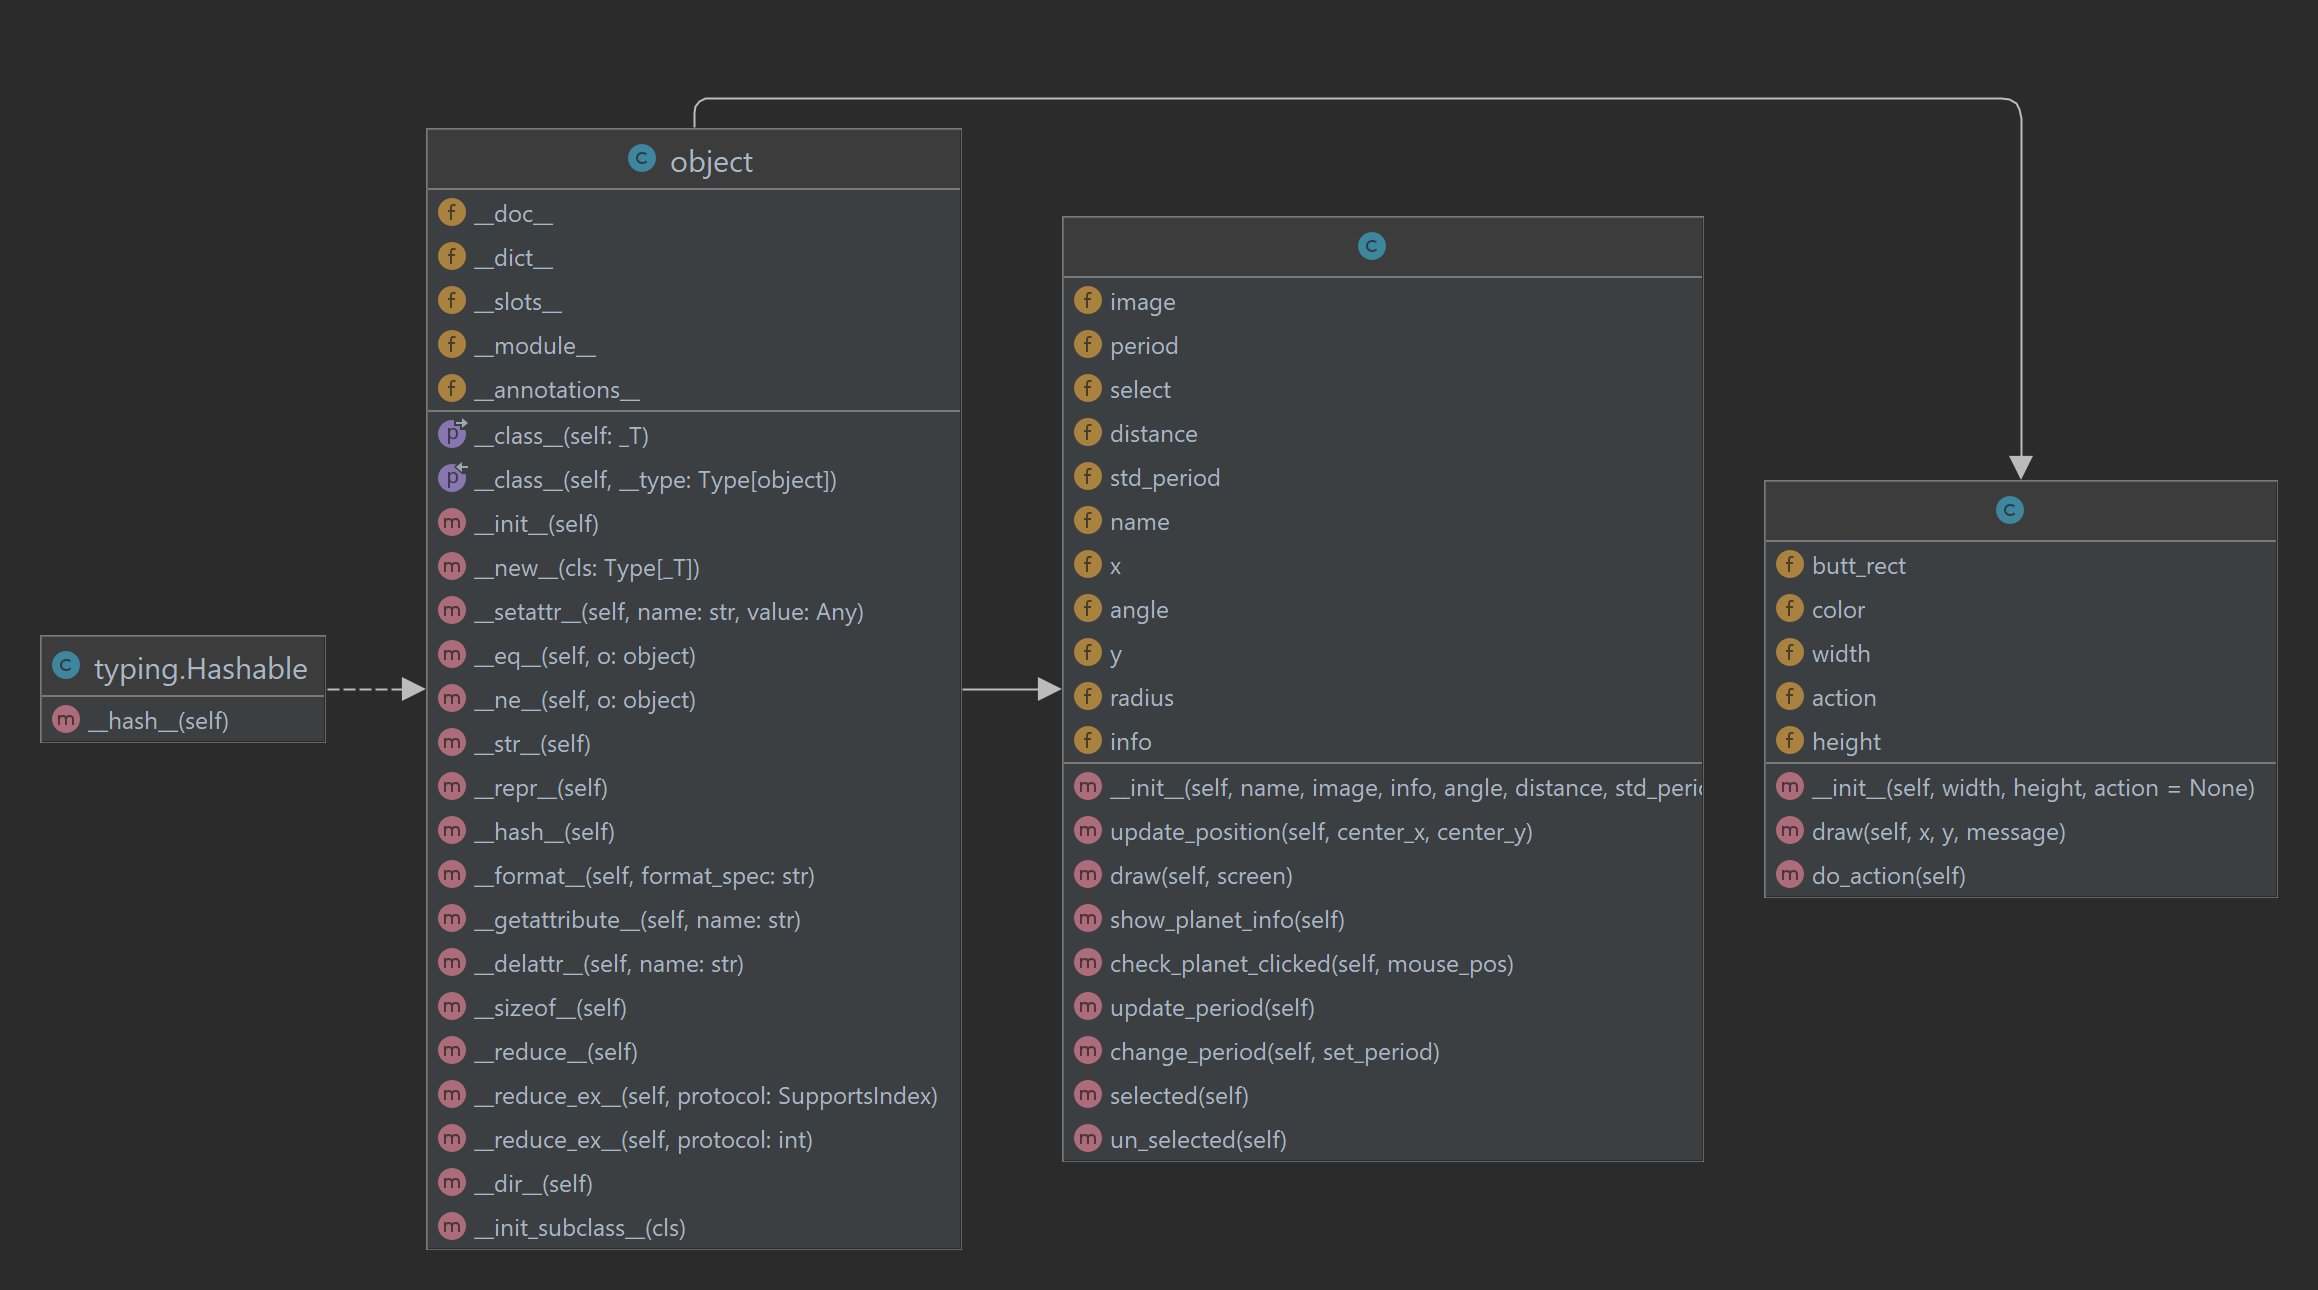
\includegraphics[width=0.8\linewidth]{src/SolarSystem.png}
\caption{Диаграмма UML, описывающая архитектуру кода программы}
\label{fig:mpr}
\end{figure}


\section{Тестирование программы}



\chapter*{Заключение}
\addcontentsline{toc}{chapter}{Заключение}
Ссылка на репозиторий проекта:~\textcolor{blue}{\url{https://github.com/davyd-off/solar-sys}}

Все члены группы оставляют commt'ы, отследить их можно по ссылке:~\textcolor{blue}{\url{https://github.com/davyd-off/solar-sys/network}}




\newpage
\addcontentsline{toc}{chapter}{Список использованной литературы}
\printbibliography[title={Список использованной литературы}]

\newpage
\chapter*{Приложение}
\addcontentsline{toc}{chapter}{Приложение}

\begin{code}
\captionof*{listing}{Код программы на языке \textit{Python3}.}\label{code:solar-sys}
\inputminted[mathescape,linenos,frame=lines,breaklines]{Python}{src/SolarSystem.py}
\end{code}
Ссылка на репозиторий проекта:~\textcolor{blue}{\url{https://github.com/davyd-off/solar-sys}}


\end{document}
